\documentclass[conference]{IEEEtran}
\IEEEoverridecommandlockouts
% The preceding line is only needed to identify funding in the first footnote. If that is unneeded, please comment it out.
\usepackage{cite}
\usepackage{pdfpages}
\usepackage{amsmath,amssymb,amsfonts}
\usepackage{algorithmic}
\usepackage{graphicx}
\usepackage{textcomp}
\usepackage{xcolor}
\usepackage{threeparttable}
\def\BibTeX{{\rm B\kern-.05em{\sc i\kern-.025em b}\kern-.08em
    T\kern-.1667em\lower.7ex\hbox{E}\kern-.125emX}}
\begin{document}

\title{Prediction of ML Operator Performance\\
}

\author{\IEEEauthorblockN{1\textsuperscript{st} Apostolos Garos}
\IEEEauthorblockA{\textit{School of ECE} \\
\textit{NTUA}\\
Athens, Greece \\
el18198@mail.ntua.gr}
\and
\IEEEauthorblockN{2\textsuperscript{nd} Nikolaos Vlachakis}
\IEEEauthorblockA{\textit{School of ECE} \\
\textit{NTUA}\\
Athens, Greece \\
el18441@mail.ntua.gr}
\and
\IEEEauthorblockN{3\textsuperscript{rd} Georgios Angelis}
\IEEEauthorblockA{\textit{School of ECE} \\
\textit{NTUA}\\
Athens, Greece \\
el18030@mail.ntua.gr}
}

\maketitle

\begin{abstract}
This paper presents a study on predicting the performance of machine learning operators in Apache Spark, with the aim of improving the efficiency of big data analytics. A multi-node Spark cluster was set up to process large datasets using the PySpark MLlib machine learning algorithms. We focused our efforts on extensively experimenting with the k-means clustering, Random Forest Regression, and Word2Vec operators. With the results we collected, we trained models that can accurately predict each operator's behavior on given dataset dimensions.
\end{abstract}

\begin{IEEEkeywords}
spark, mllib, operators, prediction
\end{IEEEkeywords}

\section{Introduction and Goals}

With the rise of big data, organizations are increasingly relying on big data analytics to extract valuable insights from large and complex datasets. Apache Spark has emerged as one of the most popular big data processing frameworks due to its ability to handle large-scale data processing and its support for a wide range of machine learning algorithms. However, executing machine learning operators in Apache Spark can be a complex and time-consuming process, which can hinder the efficiency of big data analytics.

To address this challenge, this paper proposes an innovative approach to optimize the performance of machine learning operators in Apache Spark. The approach involves using machine learning techniques to predict the performance of these operators without actually executing them. This approach is based on the idea of collecting multiple measurements of operator execution over time and using a learning algorithm to create a model that can accurately predict performance.

The main objective of this study is to provide a practical solution for improving the efficiency of big data analytics by predicting the performance of machine learning operators in Apache Spark. This paper will outline the methodology used to collect and process data, the machine learning algorithms used to create performance prediction models, and the evaluation of the proposed approach. The results of this study can help organizations optimize the performance of machine learning operators in Apache Spark, enabling them to extract insights from large and complex datasets more efficiently.

The remainder of this paper is structured as follows. Section 2 provides an overview of the steps that were followed to set up the infrastructure. Section 3 explains the systems and software products that were utilized for this study. Section 4 outlines the methodology used to create and collect data. Section 5 is an overview of the datasets that were created. Section 6 describes the process of training the final models. Finally, Section 7 presents the proposed approach's evaluation, including the prediction models' performance.

The repo at \url{https://github.com/NikosVlachakis/Information-Systems-Analysis-and-Design} contains the code developed for the purpose of executing all the steps of this study.



\section{Infrastructure Setup}

In this section, we present the steps that were followed in order to set up a multi-node cluster (1 master and 1 slave) on virtual machines (VMs) hosted in the Okeanos service. The goal was to have a running Apache Spark v3.1.3 cluster, where multiple VMs would work together to process large datasets. The steps were executed in a terminal running Ubuntu 16 LTS.

\subsection{Installation of Prerequisites}

We first set up our VMs in Okeanos, connected them to each other through a private network, and attached a public IP address to the master VM. We then connected to the VMs using the SSH protocol and started the setup process on each of them.

The first step was to install the basic tools that our cluster needed to work properly. These tools were:
\begin{itemize}
\item{\textbf{Python 3.8:} the programming language that we would use}
\item{\textbf{pip:} the Python package manager we chose to utilize}
\item{\textbf{Pyspark:} the Python library for Apache Spark}
\item{\textbf{Java:} necessary for our Apache spark cluster}

\end{itemize}

\subsection{Installation of Apache Spark}

The next step was to install Apache Spark itself. This was done by executing the following steps:
\begin{enumerate}
\item{Download the compressed source code from the official website. The specific version we installed was \textit{spark-3.1.3-bin-hadoop2.7}}
\item{Decompress the source code and place it in the destined folder in our vms}
\item{Update the textit{bashrc} file to export the necessary global variables}
\end{enumerate}

\subsection{Setup of Apache Spark cluster}

The final step was to set up the multi-node Spark cluster. 
These are the actions that were performed:

\begin{enumerate}
    \item {Set up password-less communication by exchanging ssh keys between the nodes}
    \item {Added the IP addresses of the master and slave nodes to the necessary configuration files, to ensure proper initialization and operation of the cluster}
    \item {Initialized the Spark cluster using the \textit{start-master.sh} script}
    \item {Configured one worker per VM to utilize the maximum available resources of the machine}
    \item {Deployed the workers}
\end{enumerate}


\section{System and Software Description}
In this study, we utilized the Okeanos-Knossos services for virtual machines and Apache Spark for the distributed engine. The machine learning algorithms were implemented using PySpark, the Python API for Apache Spark, and the MLlib library, which provides a wide range of machine learning algorithms. Additionally, we used the scikit-learn (sklearn) library for the development of the final model that would make predictions.

\subsection{Apache Spark}
Apache Spark \cite{spark} is a powerful platform for large-scale data processing that provides a fast and efficient way to process and analyze big data. It is designed to scale easily, allowing for the distribution of computation tasks among multiple nodes in a cluster. This enables the processing of large datasets in a timely and practical manner.

\subsection{PySpark}
PySpark \cite{pyspark} is the Python API for Apache Spark, providing a simple and convenient way to implement machine learning algorithms using Spark's distributed computing capabilities. In this study, PySpark was used in conjunction with the MLlib library, which provides a wide range of pre-implemented machine learning algorithms, including KMeans, Random Forest, and Word2Vec, which were tested.

The PySpark API allows for the implementation of machine learning algorithms in a concise and efficient manner, taking advantage of the parallel processing capabilities of Apache Spark. This makes it well-suited for large-scale machine learning applications, as it enables the processing of large datasets in a timely and practical manner.

\subsection{Virtual Machines}
In this study, virtual machines were used to provide the infrastructure for the processing tasks. The virtual machine infrastructure consisted of two virtual machines (VMs), one designated as the master node and one as the slave node.

The master node had a public IP address, allowing it to be accessed from outside the virtual machine network. This is important for managing and monitoring the processing tasks, as well as for retrieving the results of the computations. The master node communicates with the slave node through a private network, ensuring the security of the data being processed.

The slave node is responsible for executing the computation tasks assigned to it by the master node. In this study, one virtual machine was designated as the slave node, with one worker. The slave node works with the master node to process the data in a distributed manner, taking advantage of the parallel processing capabilities of Apache Spark.

\subsection{Scikit-learn Library}
The scikit-learn library \cite{{scikit-learn}} is an open-source software library for machine learning in the Python programming language. It provides a wide range of machine learning algorithms, including regression, classification, clustering, and dimensionality reduction. The library is designed to be efficient, simple, and accessible, making it a popular choice among data scientists and machine learning practitioners.

One of the key features of the scikit-learn library is its modular design, which allows for easy combination of different algorithms and techniques to build complex machine learning models. The library also provides a number of tools for model evaluation, such as cross-validation and model selection, which are important for ensuring that the models are accurate and reliable.

\section {Experiment Methodology}
The methodology that we followed to conduct our experiments and compose the dataset that was used to train our final prediction model is presented in this section. We will present the assumptions that were initially made, the problems we faced, and the conclusions that we came to while designing and implementing the scripts that would run the experiments.
\par
The goal of the current work is to create an accurate model of how each MLlib operator behaves.
Each experiment consisted of 4 main phases:
\begin{enumerate}
    \item {Initialization}
    \item {Dataset generation}
    \item {Execution}
    \item {Statistics collection}
\end{enumerate}
The statistics collected during the final phase were used to compose a dataset that consisted of data points that described the operator's behavior based on input dimensions. 


\subsection{Initialization}
In this phase, we initialized the spark session, making necessary changes to the default configuration options. The modifications were derived from a comprehensive analysis of the fundamental principles associated with each concept and its correlation with the intended application. This approach was further reinforced by the resolution of technical challenges encountered during the initial experimentation phase.

The changes that were made are:
\begin{itemize}
    \item {\textbf{spark.executor.memory = 2000 MB:} we decided one executor per VM was optimal for our case. We set the maximum amount of memory that did not interfere with the general health of the VM}
    \item \textbf{spark.executor.cores = 2:} in order to have faster computations 
    \item \textbf{spark.driver.memory = 3g:} we chose a large value because after a few trials we concluded that setting this to smaller values impacted our system's performance and chances of finishing the experiment
    \item \textbf{spark.cleaner.periodicGC.interval = 1min:} we reduced this to assist the memory cleanup process, since RAM proved to be the bottleneck of our system
\end{itemize} 


\subsection{Dataset generation}
In the course of our experiments, we determined that it would be necessary to generate our own datasets to test the various operators. This decision was based on several key factors.
\par
Firstly, accuracy and realism of the datasets were not of primary concern in our study. Instead, we were focused on evaluating the time and resources utilized during the execution of the algorithms.
\par
In addition to this, the ability to have a dynamic tool that could generate data with different dimensionalities and dataset sizes as needed was of utmost importance to our research. Gathering a diverse array of datasets from external sources to form a comprehensive pool for experimentation would have been a tedious and time-consuming process, which we sought to avoid.
\par
To achieve the best results, we created a dedicated generator for each operator we tested. These generators took the number of samples and number of features as inputs, and generated the desired datasets. The resulting datasets were saved in predefined files on disk, and the corresponding metadata were saved in a separate file. These metadata consisted of information such as the number of rows, the number of columns, the number of clusters (when applicable), and the size of the dataset in megabytes.
\par
More specifically, following our experimentation, we arrived at the conclusion that for the KMeans and RandomForest algorithms, it would be optimal to utilize the \textit{make\textunderscore blobs} and \textit{make\textunderscore regression} functions from the \textit{sklearn.datasets} package to generate the datasets, and the \textit{dump\textunderscore svmlight\textunderscore file} function from the same package to save them in the \textit{libsvm} format. We integrated them in our data generator scripts and extended their functionality using a batching approach in order to be able to create large datasets efficiently and without failures.
\par
In the case of the word2vec operator, we devised a bespoke data generator that followed the same principles as the others. However, it did not incorporate any external tool for data creation. Given that the word2vec operator requires a distinct type of data, we generated datasets in the form of sentences, with each sentence occupying a single row in the dataset. The sentences were generated by randomly selecting words from a dictionary of 200 unique words that we created. This method of sentence generation is valid in our scenario as the coherence of the sentences is not essential for the proper functioning of the word2vec algorithm. To maintain a consistent dimensional structure across different tests, we determined that all sentences should contain the same number of words. The resulting dataset was saved in the CSV format.

\par
Overall, our decision to generate our own datasets allowed us to have a high degree of control over the experiments and to test the algorithms in a variety of scenarios, which was critical to our research.


\subsection{Execution}
The implementation of the experimental component of this study was relatively straightforward. The primary consideration was determining the parameters of the experiments, specifically selecting the range for both the number of rows and columns to be used as dimensions in the test datasets. After numerous experiments, we concluded that, given our limited resources, there should be a significantly lower limit on the number of columns, but the number of rows rising was not a concern. 
The limits we selected for each operator were:

\begin{table}[h!]
\centering
\begin{tabular}{|c|c|c|c|}
\hline
\textbf{Operator} & \textbf{Number of rows range} & \textbf{Number of columns range} \\ \hline
KMeans & 10\textsuperscript{2}-10\textsuperscript{7} & 2-100 \\ \hline
Random forest & 10\textsuperscript{2}-10\textsuperscript{6} & 10-100 \\ \hline
Word2Vec & 10\textsuperscript{2}-5*10\textsuperscript{6} & 3-50 \\ \hline
\end{tabular}
\caption{Experimental parameters for different operators.}
\label{table:experimental_parameters}
\end{table}

The KMeans operator had one more feature, the number of centers, with a range of 2-20.
A unique consideration was made for the range of columns in the word2vec experiment. The upper limit was not established through experimental evaluation or performance considerations. To maintain a degree of realism, we conducted research on the average sentence length in the English language and found that it falls within the range of 15-20 words \cite{acropolitan}. In light of this, we chose the upper limit to be slightly larger, settling on 50 as the value.
\par
The models utilized in the execution phase were obtained from the PySpark library, with default values for all parameters, with the exception of the kmeans model, where the number of centers was dynamically set. In order to ensure efficient experiment execution, the maximum number of iterations was fixed at 10. This decision was based on previous experiences where training failed to converge, causing significant disruption to the experiment process.
\par
Finally, the model was fit to the experimental dataset. However, no predictions or scoring were carried out as they fall outside the scope of this study.
Throughout the majority of the tests, the CPU and memory usage of the Spark clusters and VMs were closely monitored. Our observations indicated that memory was the primary constraint in the system. To address this issue, we made sure to consistently delete all variables and unpersist the datasets, effectively reducing the burden on memory.

\subsection{Statistics collection}
The final phase of each experiment involved monitoring, logging, and preserving relevant statistics that would aid in the training of the final prediction model. This is where the final datasets used for model training were created.
\par
Initially, the dimensions of the experimental dataset were saved, including the number of samples, features, and size in megabytes. For datasets utilized in testing the kmeans algorithm, the number of clusters was also recorded. These features would be required input for the prediction model in order to produce an estimate of the operator's behavior.
\par
From the statistics collected on the operator execution, three key metrics were analyzed: training time, memory usage, and CPU utilization. These values were monitored using logs and the Spark UI, and informed important decisions that shaped the direction of the rest of the study.
\par
With regards to CPU utilization, after monitoring the VMs during test executions for all operators, we observed that in both VMs, the CPU usage was consistently at a level of approximately 55-60\% throughout all executions. Given the minimal variance in this metric and the fact that it was not a bottleneck or a determining factor in the operator's performance, we decided not to save and use it in predictions.
\par
The total training time was measured using Python and included only the time taken by the operator to fit the data.
\par
After the completion of the model fitting process, we retrieved the memory utilization data from the cluster. To obtain this information, we accessed the REST API of the Spark UI and retrieved data regarding all executors that were utilized during the execution of the Spark application. Subsequently, we aggregated the "memoryUsed" field to calculate the total memory consumption of the entire cluster.
\par
In conclusion, the results of this study showed that the training time and memory usage were the most representative values of each operator's behavior. These metrics were chosen as the targets in our final prediction model, as they have a direct impact on the performance and efficiency of the operator. By using these statistics, we aim to accurately estimate the operator's behavior and optimize the execution of the Spark application. 

\section{Experiment results}
After conducting a substantial number of experiments for each operator, we have obtained a significant amount of results. These results are stored in individual datasets for each operator, which will be utilized to train the prediction models in the final stage of this study.

Each dataset comprises seven columns with the following names:

\begin{enumerate}
    \item {\textbf{Total Time:} the time that the operator took to fit the data}
    \item {\textbf{Memory Usage:} the amount of memory used by the cluster}
    \item {\textbf{num\_samples:} the number of samples in the dataset}
    \item {\textbf{num\_features:} the number of features in each sample}
    \item {\textbf{num\_classes:} the number of clusters in the dataset (only present in the kmeans dataset)}
    \item {\textbf{dataset\_size:}} the size of the dataset in megabytes
\end{enumerate}

The first two columns will be used as targets in the final model, while the others will be the input features. 

In order to gain a deeper understanding of our datasets and optimize our model training, we conducted a thorough analysis of the data and created visualizations for each input-target pair.
These visualizations provided us with valuable insights into the patterns and trends present in the data, and helped us identify the most relevant features for predicting the target variables.
By leveraging this information, we can develop highly accurate and efficient prediction models that will allow us to make informed decisions and take appropriate actions.

\subsection{KMeans}


\subsubsection{\textbf{Total Time}}

Through the visualizations, it is evident that the data points are well-distributed without many outliers, making them suitable for training a prediction model.

\begin{figure}[ht]
  \centering
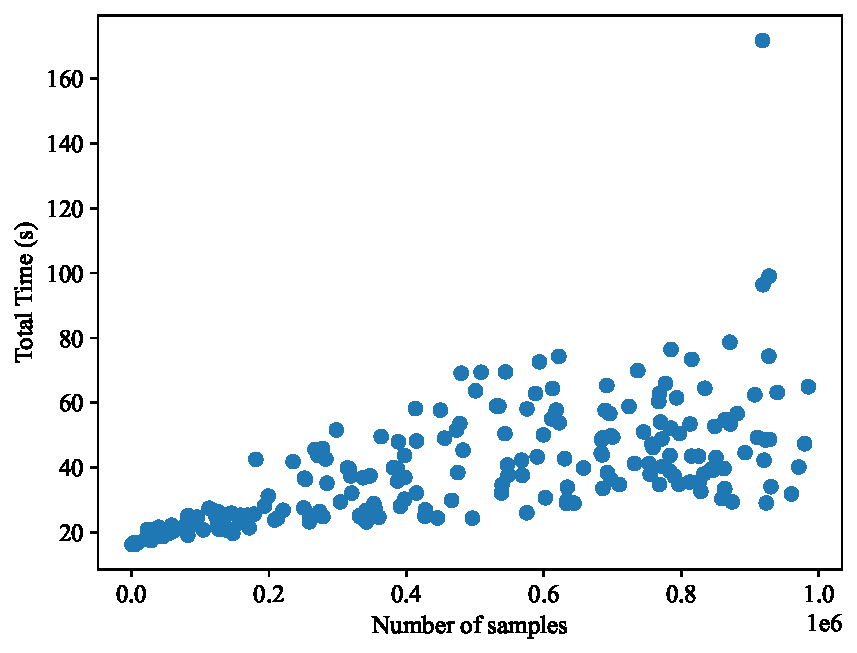
\includegraphics[width=0.4\textwidth]{plots/experiment_results/kmeans_time_samples.pdf}
  \caption{Total Time and Number of Samples relationship}
\end{figure}

\begin{figure}[ht]
    \centering
  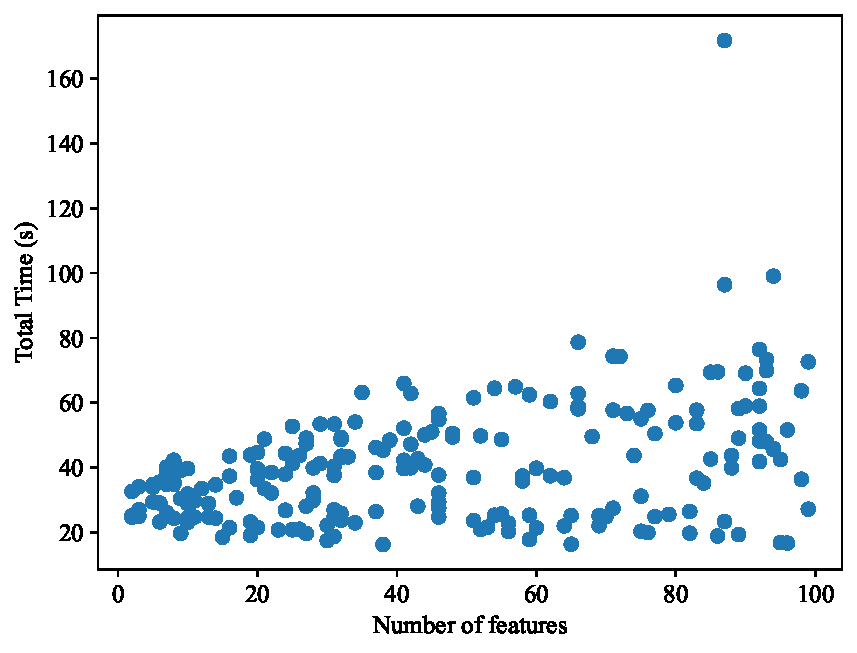
\includegraphics[width=0.4\textwidth]{plots/experiment_results/kmeans_time_features.pdf}
    \caption{Total Time and Number of Features relationship}
  \end{figure}

The visualizations for the time distributions with respect to the number of samples and features showcase a key characteristic that makes them ideal for training prediction models with proper preprocessing. Specifically, both distributions exhibit a linearly growing upper limit and a consistent lower limit.

The presence of a linearly growing upper limit in the distributions implies that as the number of samples or features increases, the total time taken for training also increases proportionally. This is a desirable property since it indicates that the model is able to scale well with larger datasets. Additionally, the consistent lower limit of the distributions means that even with smaller datasets, the total time required for training is still significant enough to train the model accurately. This is essential for achieving accurate predictions even with limited data.

The fact that both distributions exhibit these properties makes them highly valuable for training prediction models. However, it is important to note that proper preprocessing techniques should be employed to optimize the training process and achieve the best possible results.

\begin{figure}[ht]
    \centering
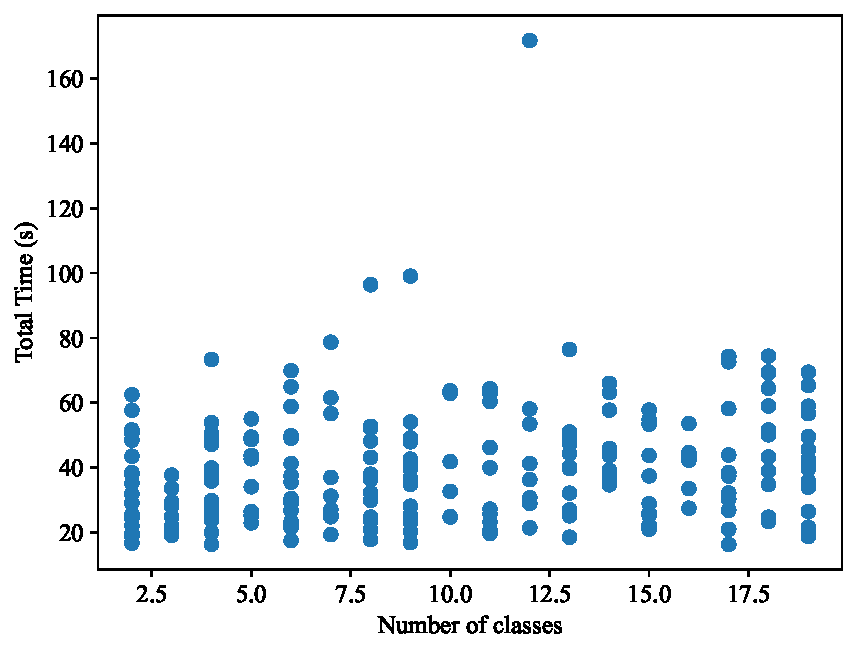
\includegraphics[width=0.4\textwidth]{plots/experiment_results/kmeans_time_classes.pdf}
    \caption{Total Time and Number of Clusters relationship}
    \end{figure}
The "Total time - Number of clusters" visualization reveals an almost uniform distribution, indicating that the cluster number is not significantly correlated with the time taken for the training algorithm to converge. As a result, it will have a low weight on the final predictions or will be eliminated prior to training.

\begin{figure}[ht]
    \centering
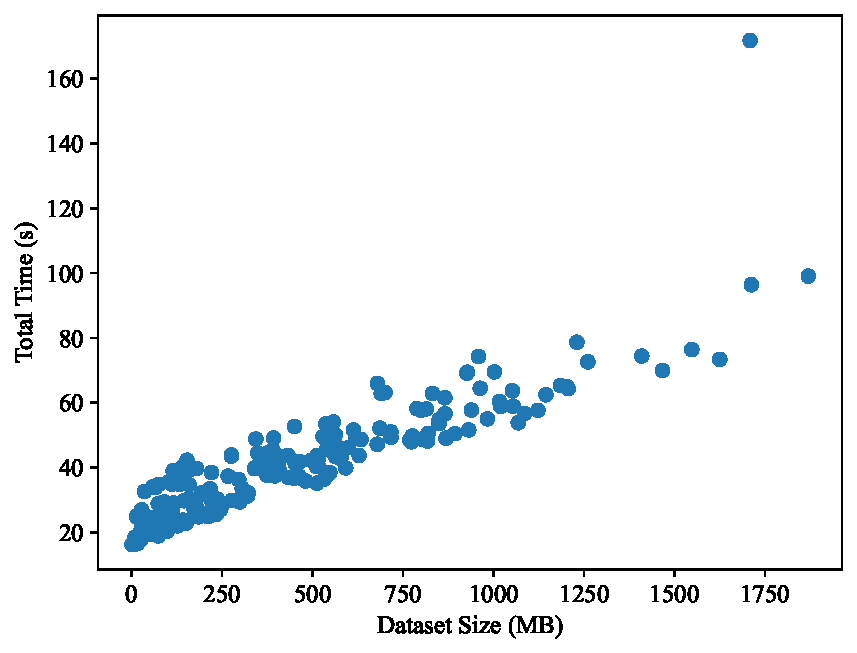
\includegraphics[width=0.40\textwidth]{plots/experiment_results/kmeans_time_dataset_size.pdf}
    \caption{Total Time and Dataset Size relationship}
\end{figure}


The "Total time - Dataset size" plot illustrates an almost linear relationship between the two values, highlighting the importance of preserving this column in the data preprocessing phase.

\bigskip

\subsubsection{\textbf{Memory Usage}}

When analyzing the visualizations related to the Memory Usage target column, we observe that there are some similarities to the previous target column, but also some important differences.

Like the previous target column, the visualizations for Memory Usage show a generally well-distributed set of data points without many outliers, which is a positive sign for model training. However, it is important to consider the unique characteristics of each target column and design appropriate modeling and preprocessing strategies accordingly



\begin{figure}[ht]
    \centering
  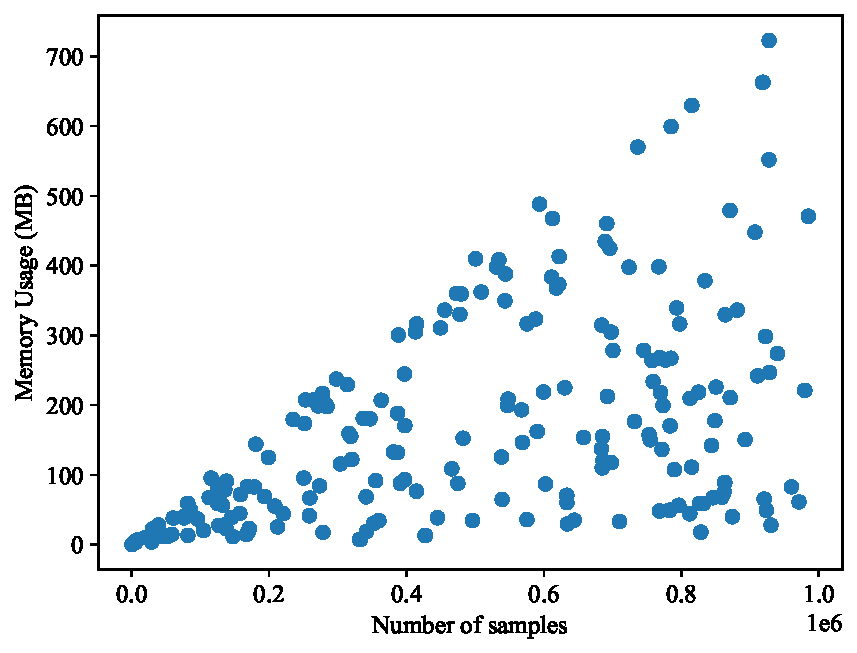
\includegraphics[width=0.4\textwidth]{plots/experiment_results/kmeans_memory_samples.pdf}
    \caption{Memory Usage and Number of Samples relationship}
  \end{figure}
  
  \begin{figure}[ht]
      \centering
    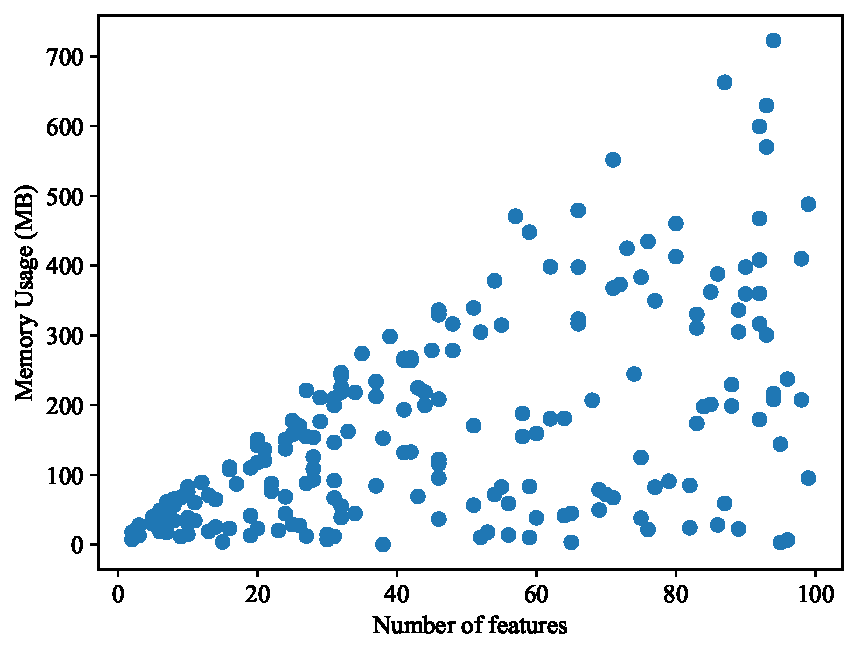
\includegraphics[width=0.4\textwidth]{plots/experiment_results/kmeans_memory_features.pdf}
      \caption{Memory Usage and Number of Features relationship}
    \end{figure}

Like the Total Time distributions, the Memory Usage distributions demonstrate a growing upper limit as the number of samples or features increases. However, the patterns in these distributions tend to be more complex, exhibiting a faster growth in Memory Usage with increasing number of samples or features. This leads to a wider range of Memory Usage values for larger datasets compared to smaller ones, making it more challenging to predict the Memory Usage required for a given task accurately.

It is worth highlighting that, while the Memory Usage distribution with regards to number of samples and number of features appears to be more complex and challenging to fit compared to the Total Time distribution, it is still within acceptable margins. This means that the column containing Memory Usage values will still be highly valuable for training prediction models, especially with appropriate preprocessing techniques.



  \begin{figure}[ht]
      \centering
      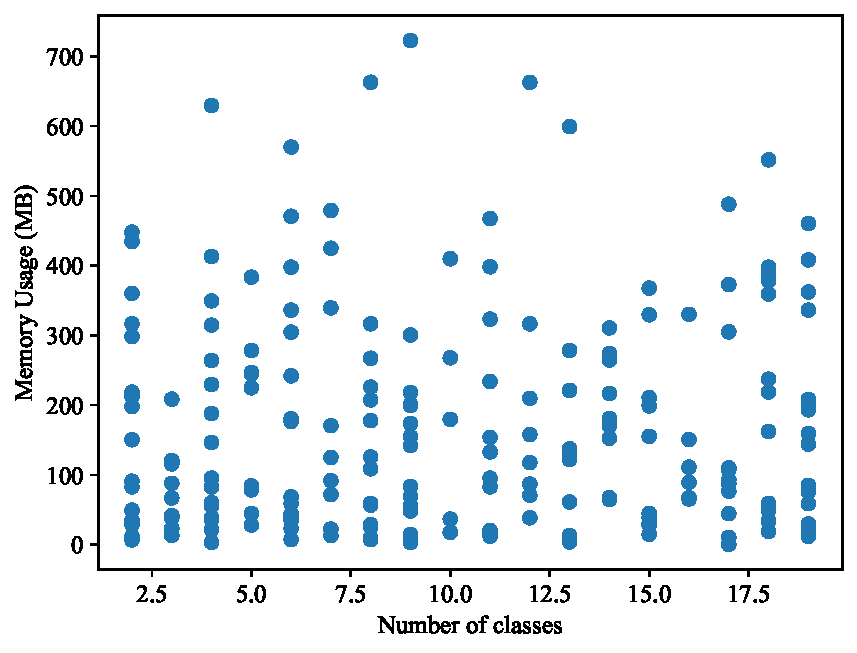
\includegraphics[width=0.4\textwidth]{plots/experiment_results/kmeans_memory_classes.pdf}
      \caption{Memory Usage and Number of Clusters relationship}
      \end{figure}

As was the case when we visualized the Time Taken and Number of clusters relationship, the distribution does not reveal a pattern that can help us train a model. In this case, we have an even bigger spread in values. The num\_classes column will not be very helpful in the fitting of the final model.

  \begin{figure}[ht]
      \centering
  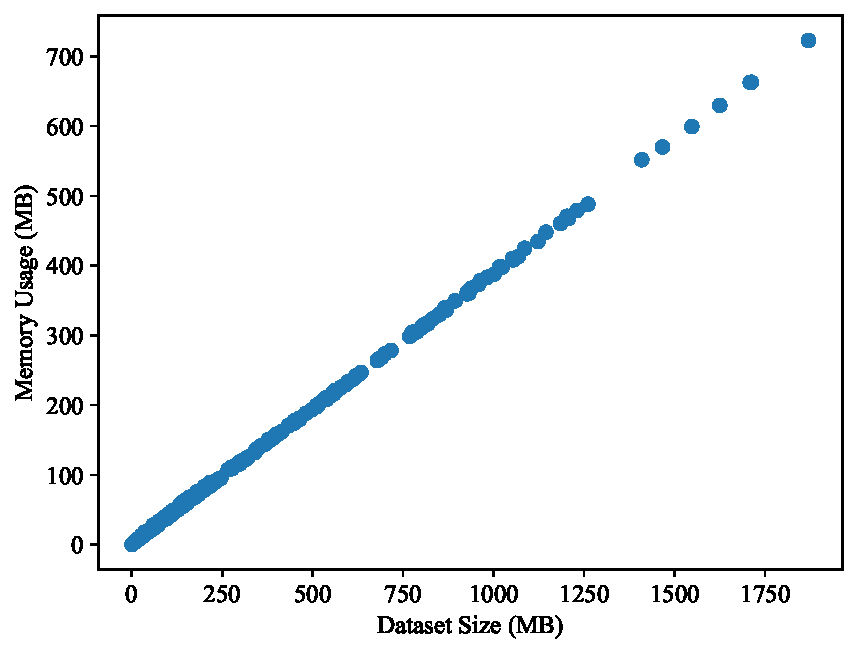
\includegraphics[width=0.4\textwidth]{plots/experiment_results/kmeans_memory_dataset_size.pdf}
      \caption{Memory Usage and Dataset Size relationship}
  \end{figure}

\bigbreak
  The "Memory usage - Dataset size" plot show an almost perfect linear relationship between the dataset size and the Memory Usage. This means this column will be very important in our final model training. 
  

\subsection{Random Forest}

Upon further analysis of the random forest dataset, we can observe that it shares several similarities with the kmeans dataset that we analyzed previously. The size of the dataset is still a critical feature, as it exhibits a well-defined relationship with the target variables. Therefore, we can conclude that the size of the dataset is a crucial aspect to consider when training our model.

However, we can also note that the other input variables in the dataset can offer valuable insights and play a critical role in training the model. These variables may not exhibit a clear relationship with the target variables, but they can provide additional information that can help our model make more accurate predictions.

It is essential to note that there are some inconsistencies in the dataset that may negatively impact our model's accuracy. Therefore, we need to carefully analyze the data to identify and address these inconsistencies. Failure to do so can result in a model that performs poorly and produces inaccurate predictions. Hence, it is crucial to preprocess and clean the data to ensure that it is suitable for training our model.

While analyzing the random forest dataset, we can observe that there are a few outliers present in the dataset. However, these outliers are relatively insignificant, considering the vast number of normal data points available. Therefore, these outliers are unlikely to have a significant impact on the model's overall performance.



It is important to mention that, in contrast to the kmeans dataset, there is no num\_classes column, as the Random Forest regressor doesnt need clusters or classes.

\subsubsection{\textbf{Time Taken}}
 The following figures visualize the Time Taken metric.
\begin{figure}[ht]
    \centering
  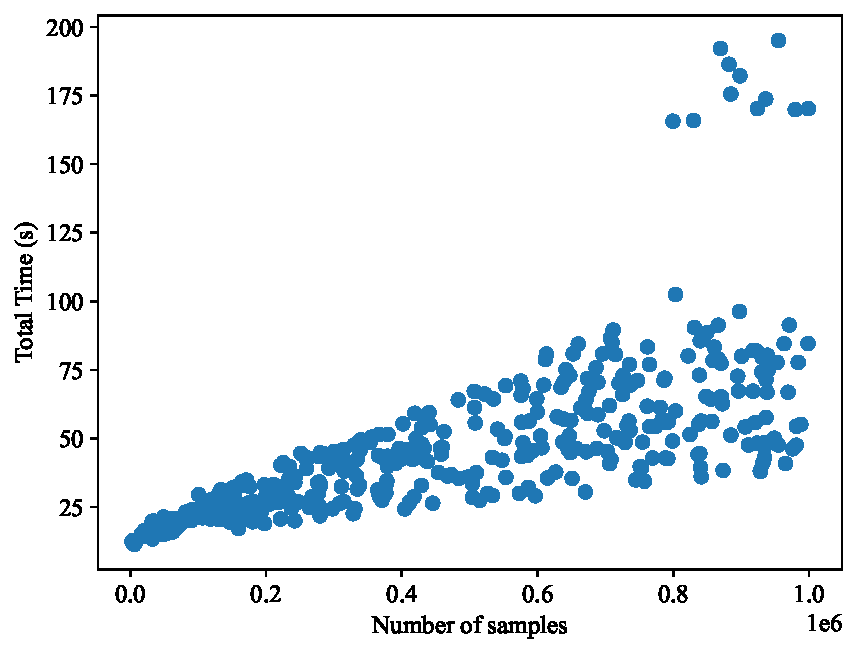
\includegraphics[width=0.4\textwidth]{plots/experiment_results/random_forest_time_samples.pdf}
    \caption{Time Taken and Number of Samples relationship}
  \end{figure}
  
  \begin{figure}[ht]
      \centering
    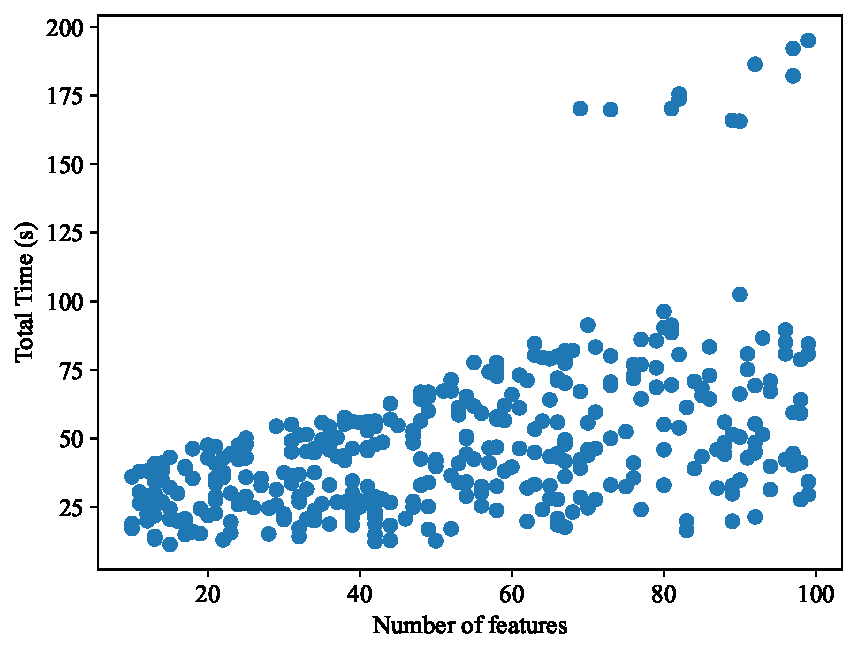
\includegraphics[width=0.4\textwidth]{plots/experiment_results/random_forest_time_features.pdf}
      \caption{Time Taken and Number of Features relationship}
    \end{figure}


Upon visualizing the data, we can once again notice the presence of an upper limit that grows steadily over time. However, what sets this dataset apart is the observation of a lower limit that also grows, albeit at a slower rate than the upper limit. This lower limit effectively restricts the spread of the Time Taken values, which can help to simplify the task of fitting a regression model.

      
  \begin{figure}[ht]
      \centering
  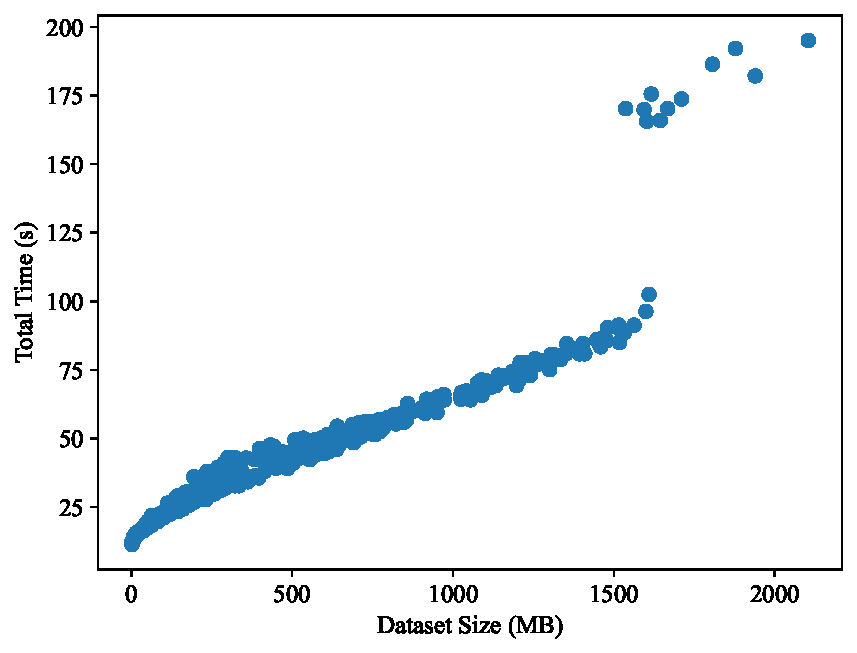
\includegraphics[width=0.4\textwidth]{plots/experiment_results/random_forest_time_dataset_size.pdf}
      \caption{Time Taken and Dataset Size relationship}
  \end{figure}

  The "Total Time and Dataset Size" relationship is once again well defined. Even though it is not linear, with some preprocessing it will be a great asset for model training

\vfill
\subsubsection{\textbf{Memory Usage}}
The Memory usage graphs show a slightly different picture of the data.

\begin{figure}[h]
\centering
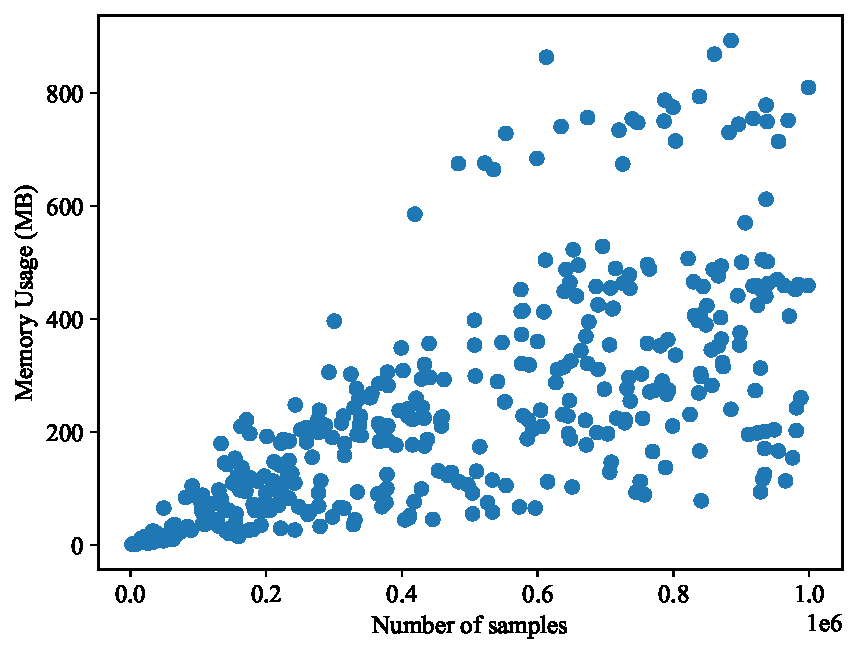
\includegraphics[width=0.4\textwidth]{plots/experiment_results/random_forest_memory_samples.pdf}
\caption{Memory Usage and Number of Samples relationship}
\end{figure}

\begin{figure}[h]
    \centering
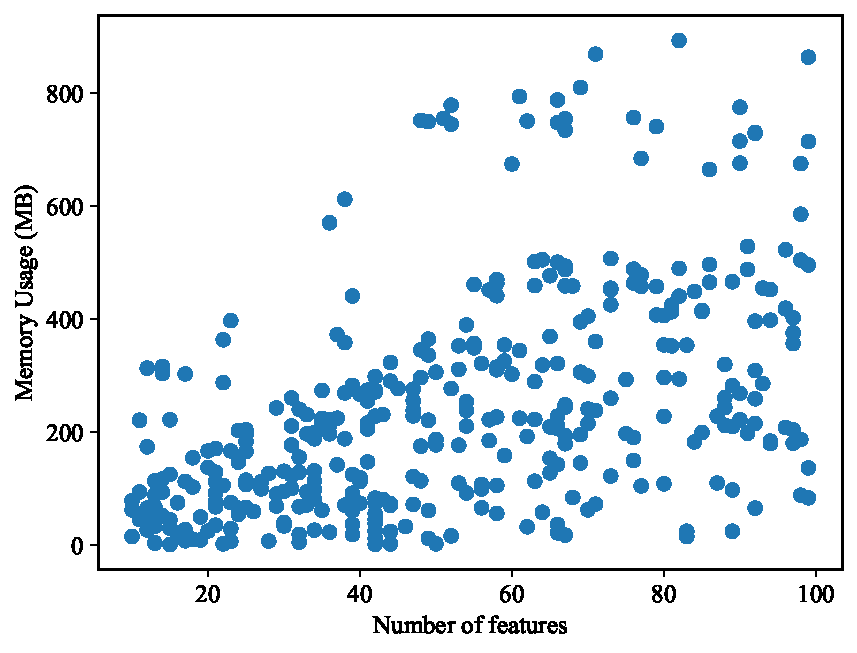
\includegraphics[width=0.4\textwidth]{plots/experiment_results/random_forest_memory_features.pdf}
    \caption{Memory Usage and Number of Features relationship}
\end{figure}

% The visualization with regard to the Number of samples and features follows the same "growing upper limit" trend, but there are many outliers. The number seems to be small, compared to the size of the dataset, but it is not something that will not affect the resulting model.

In this case, it appears that the number of samples and features follows a "growing upper limit" trend, which suggests that the dataset is increasing in size and complexity. However, the presence of many outliers may indicate that there are some anomalies or irregularities in the data that need to be addressed. These outliers could be the result of errors in data collection or processing, or they could be legitimate data points that are significantly different from the rest of the data.

Overall, while the presence of outliers and a small number of samples may present some challenges, they are not insurmountable and should not significantly affect the resulting model. By carefully analyzing and addressing any anomalies in the data and selecting appropriate methods and algorithms, it is possible to build an accurate and reliable machine learning model.





\begin{figure}[!h]
    \centering
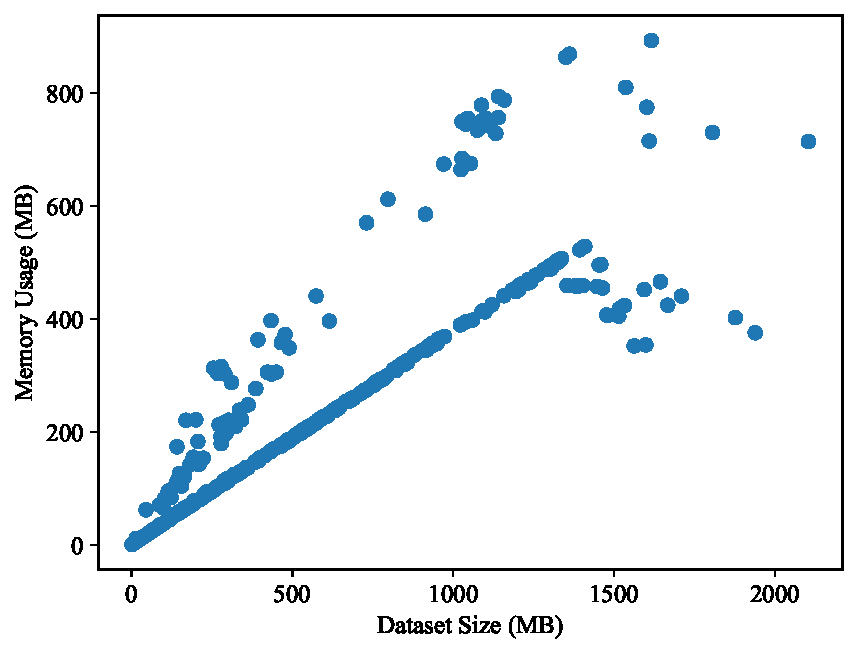
\includegraphics[width=0.4\textwidth]{plots/experiment_results/random_forest_memory_dataset_size.pdf}
    \caption{Memory Usage and Dataset Size relationship}
\end{figure}

The dataset size visualization shows us a slightly different picture compared to other cases. While there seems to be a linear relationship, there is a vast amount of data points that differ.

\vfill

\subsection{Word2Vec dataset}

Upon analyzing the dataset corresponding to the word2vec operator, we can observe that it differs significantly from the other two datasets. One of the most apparent differences is that the values on the Time Taken and Memory Usage axes will be much larger in comparison. This difference can be attributed to the inherent nature of the word2vec algorithm, which operates on large volumes of text data and involves complex computations.


\subsubsection{\textbf{Time Taken}}
The Time Taken graphs for the Word2Vec operator.

\begin{figure}[ht]
\centering
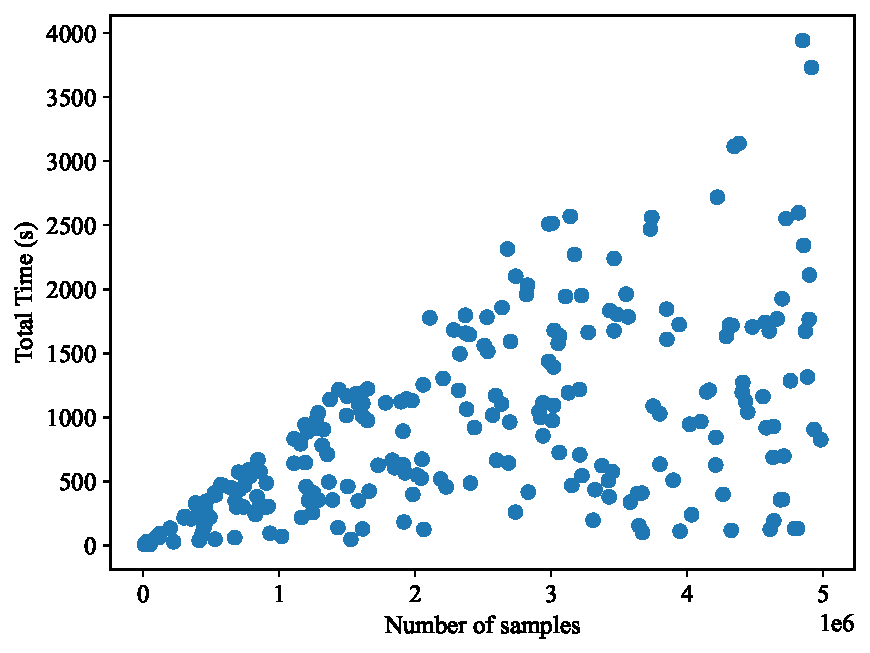
\includegraphics[width=0.4\textwidth]{plots/experiment_results/word2vec_time_samples.pdf}
\caption{Time Taken and Number of Samples relationship}
\end{figure}

\begin{figure}[ht]
    \centering
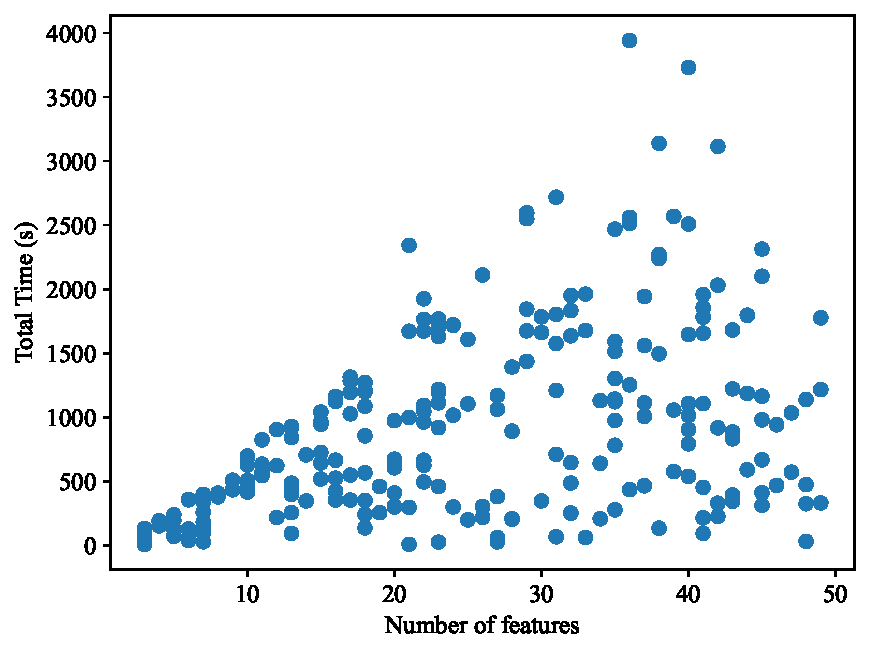
\includegraphics[width=0.4\textwidth]{plots/experiment_results/word2vec_time_features.pdf}
    \caption{Time Taken and Number of Features relationship}
\end{figure}

The Number of samples and Number of features plots are similar to the ones we have already seen. Very few outliers are observed, so we are expecting a relatively easy training process with a good result.

\begin{figure}[!h]
    \centering
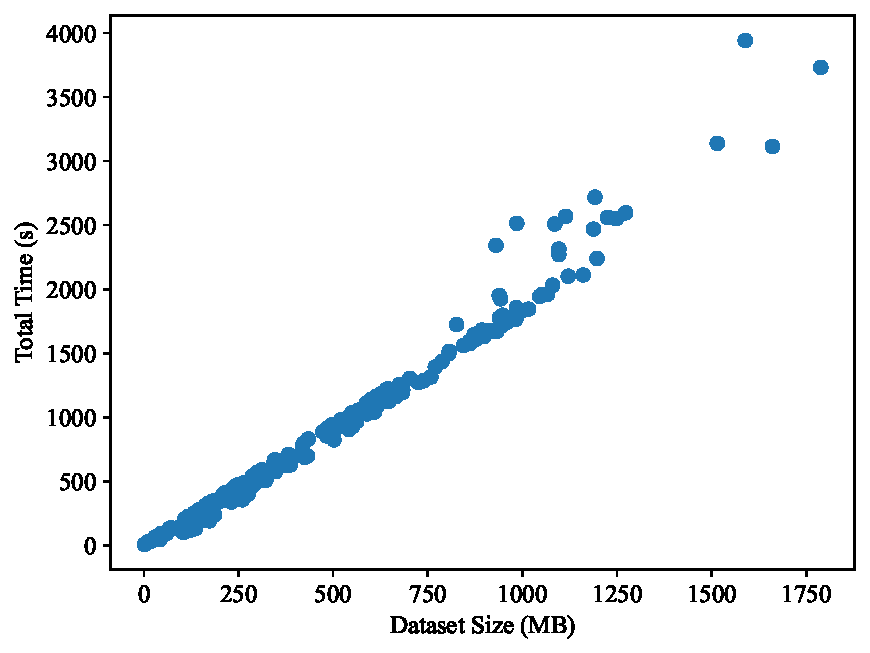
\includegraphics[width=0.4\textwidth]{plots/experiment_results/word2vec_time_dataset_size.pdf}
    \caption{Time Taken and Dataset Size relationship}
\end{figure}

The Dataset size visualization is once again almost linear. As we have analyzed before, this column will be very important in the prediction process.

\vfill
\subsubsection{\textbf{Memory Usage}}
The Memory Usage visualizations, with regards to the input columns.

\begin{figure}[hb]
\centering
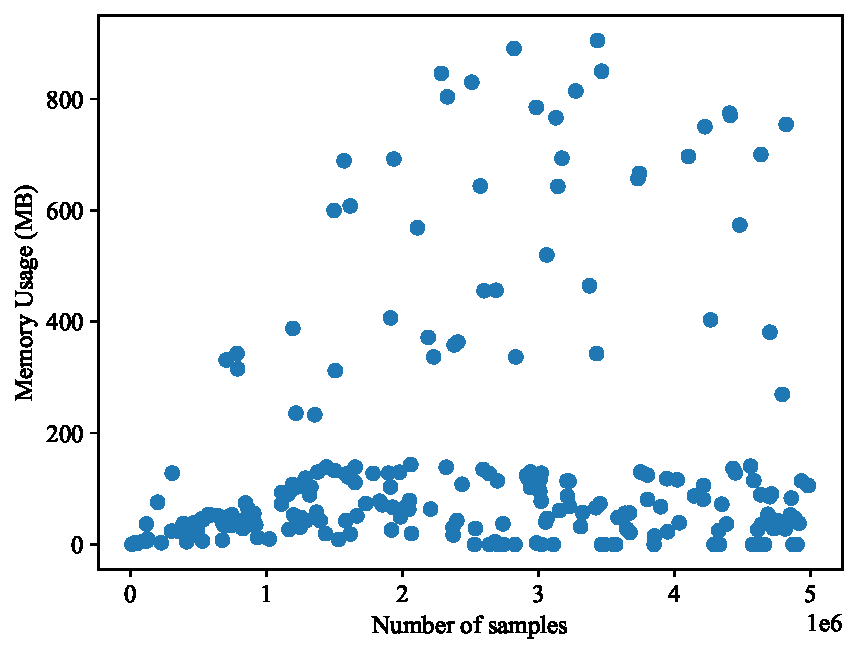
\includegraphics[width=0.4\textwidth]{plots/experiment_results/word2vec_memory_samples.pdf}
\caption{Memory Usage and Number of Samples relationship}
\end{figure}
 
\begin{figure}[ht]
    \centering
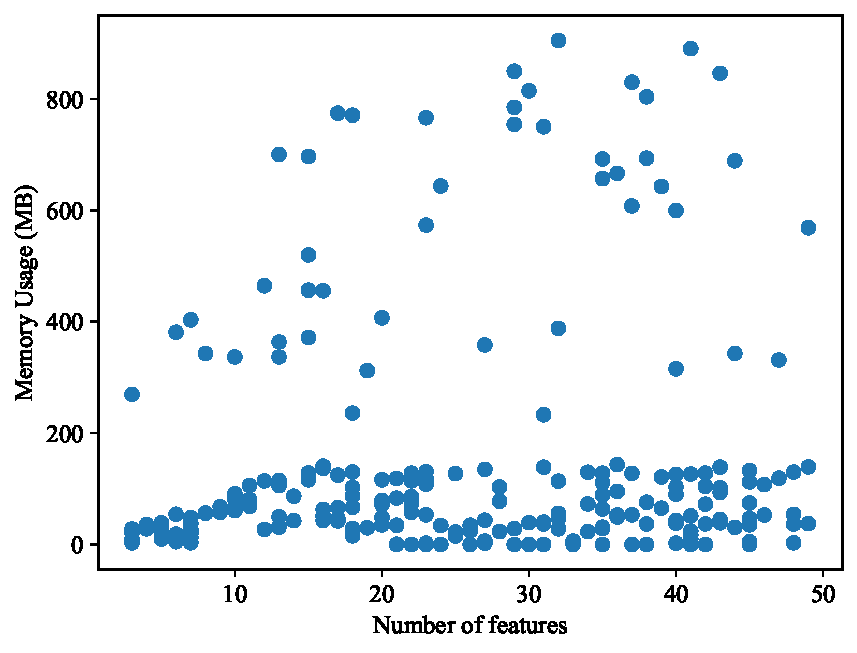
\includegraphics[width=0.4\textwidth]{plots/experiment_results/word2vec_memory_features.pdf}
\caption{Memory Usage and Number of Features relationship}
\end{figure}


The datapoints in the Number of samples and Number of features visualizations are different to what we have already seen. There is an almost uniform distribution, where many outliers are present. In the state that the datapoints are now, it is very unlikely that they can be used to train an accurate model.

The "Memory Usage and Dataset Size relationship" is not linear, like it was the case in many other visualisations. While it is not uniform or random, there is a clear spread to Memory usage values, even for datasets that have really close Dataset size properties.

\begin{figure}[!ht]
    \centering
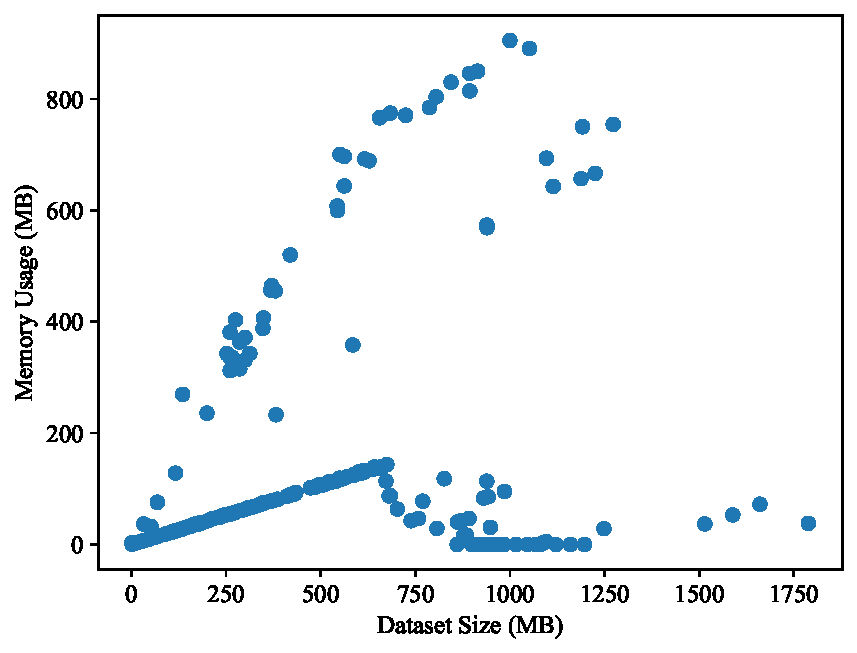
\includegraphics[width=0.4\textwidth]{plots/experiment_results/word2vec_memory_dataset_size.pdf}
    \caption{Memory Usage and Dataset Size relationship}
\end{figure}

Based on the observations made on the word2vec dataset, it is likely that creating a model that can accurately predict the Memory Usage of the word2vec operator would be a challenging task, even with proper data preprocessing and extensive experimentation with different model architectures and hyperparameters.


This difficulty can be attributed to the inherent nature of the word2vec algorithm, which involves a significant amount of randomness in its computations. This randomness can result in inconsistencies in the data, making it challenging to develop a robust and accurate model that can account for these variations.


Therefore, it may be necessary to accept a certain level of uncertainty and imprecision when predicting Memory Usage for the word2vec operator


\section{FINAL MODEL SELECTION}

In this section, we will discuss the various steps involved in the final model selection process for our regression problem. Our goal is to identify the most suitable model that can accurately predict the target variables given the input features. We will be covering the data preprocessing steps, regression model experimentation, the use of MultiOutputRegressor and Pipeline, GridSearch, and a comparison of model performance.

\subsection{Data Preprocessing}

Before building a regression model, it is crucial to preprocess the data to ensure that it is in the correct format and structure for modeling. The preprocessing of data involves several steps that aim to clean, transform and standardize the data.

In this study, the data preprocessing steps included imputation to handle missing values, feature scaling to ensure that all features are on the same scale, and variance analysis to identify if there were any highly correlated features that needed to be removed.

These steps are critical in preparing the data for modeling and can significantly impact the performance of the final model. In this study, the data preprocessing steps were carefully executed to ensure that the data was in the best possible format for model building.

\subsubsection{Imputation}
In this step, we handled missing values in the dataset by replacing them with the median of the respective column.

\subsubsection{Feature Scaling}
In this step, we scaled the features to ensure that all features were on the same scale. This helped improve the performance of the regression model and prevented any feature from dominating the model. MinMaxScaler was used to perform feature scaling. This method scales the features to a specific range between 0 and 1, making it useful for standardizing the data and preventing any feature from dominating the model.

\subsubsection{Variance Analysis}
In our analysis, we used a feature selector that removed all low-variance features. This was an important step in our process, as low-variance features often do not contribute much to the overall prediction and can even harm the performance of the model. By removing these features, we aimed to simplify the model and improve its accuracy by focusing on the most important features.

\subsection{Regression Models Experimentation}
In this section, we conducted an experiment to evaluate different regression models and determine the best performing model for our dataset. The regression models we experimented with included Random Forest Regressor, Linear Regression, Elastic Net, and Gradient Boosting Regressor.

\subsubsection{MultiOutputRegressor}

We used MultiOutputRegressor as a wrapper for each of the regression models to handle the case of multiple target variables. This was useful in our case because we wanted to predict both memory usage and total time for each training instance. The MultiOutputRegressor allowed us to train a single model that could predict both target variables simultaneously, thus reducing the complexity of the modeling process.

\subsubsection{Pipeline}

To simplify the process and make it more efficient, we used a pipeline to combine all the steps involved in the model selection process, including data preprocessing, regression model experimentation, and the use of MultiOutputRegressor.

\subsubsection{GridSearch}

We utilized GridSearch to optimize the hyperparameters of our models and find the optimal parameters that would result in the best performance. We employed a parameter grid to look for the best parameters for each of the models and utilized the GridSearchCV function from sklearn.model\_selection to conduct the search.
We used the following parameters for each model:


\begin{itemize}
\item \textbf{Random Forest:}
\begin{itemize}
\item n\_estimators: The number of trees in the forest
\item max\_depth: The maximum depth of each tree
\item max\_features: The number of features to consider when looking for the best split
\item criterion: The function to measure the quality of a split
\end{itemize}
\item \textbf{Linear Regression:}
\begin{itemize}
    \item fit\_intercept: Whether to calculate the intercept for this model
    \item normalize: Whether to normalize the regressors before fitting the model
    \item copy\_X: Whether to copy X before fitting the model
\end{itemize}

\item \textbf{Elastic Net:}
\begin{itemize}
    \item alpha: The regularization parameter
    \item l1\_ratio: The mixing parameter for L1 and L2 regularization
    \item max\_iter: The maximum number of iterations for the solver
\end{itemize}

\item \textbf{Gradient Boosting:}
\begin{itemize}
    \item n\_estimators: The number of boosting stages to perform
    \item learning\_rate: The learning rate to shrink the contribution of each tree
    \item max\_depth: The maximum depth of each tree
\end{itemize}
\end{itemize}





\subsection{Model Performance Comparison}

We compared the performance of different models by evaluating metrics such as mean absolute error and R-squared. The R-squared metric measures the proportion of the variance in the dependent variable that is predictable from the independent variable, while the mean absolute error (MAE) measures the average absolute difference between the predicted and actual values.

\subsubsection{Random Forest Regression}
We plotted the R2 scores and mean absolute error (MAE) results in separate graphs. As seen in the graph for total time, the Random Forest Regressor achieved the highest R2 score, closely followed by the Gradient Boosting Regressor. The other models lagged significantly behind in terms of performance.

\begin{figure}[ht]
  \centering
  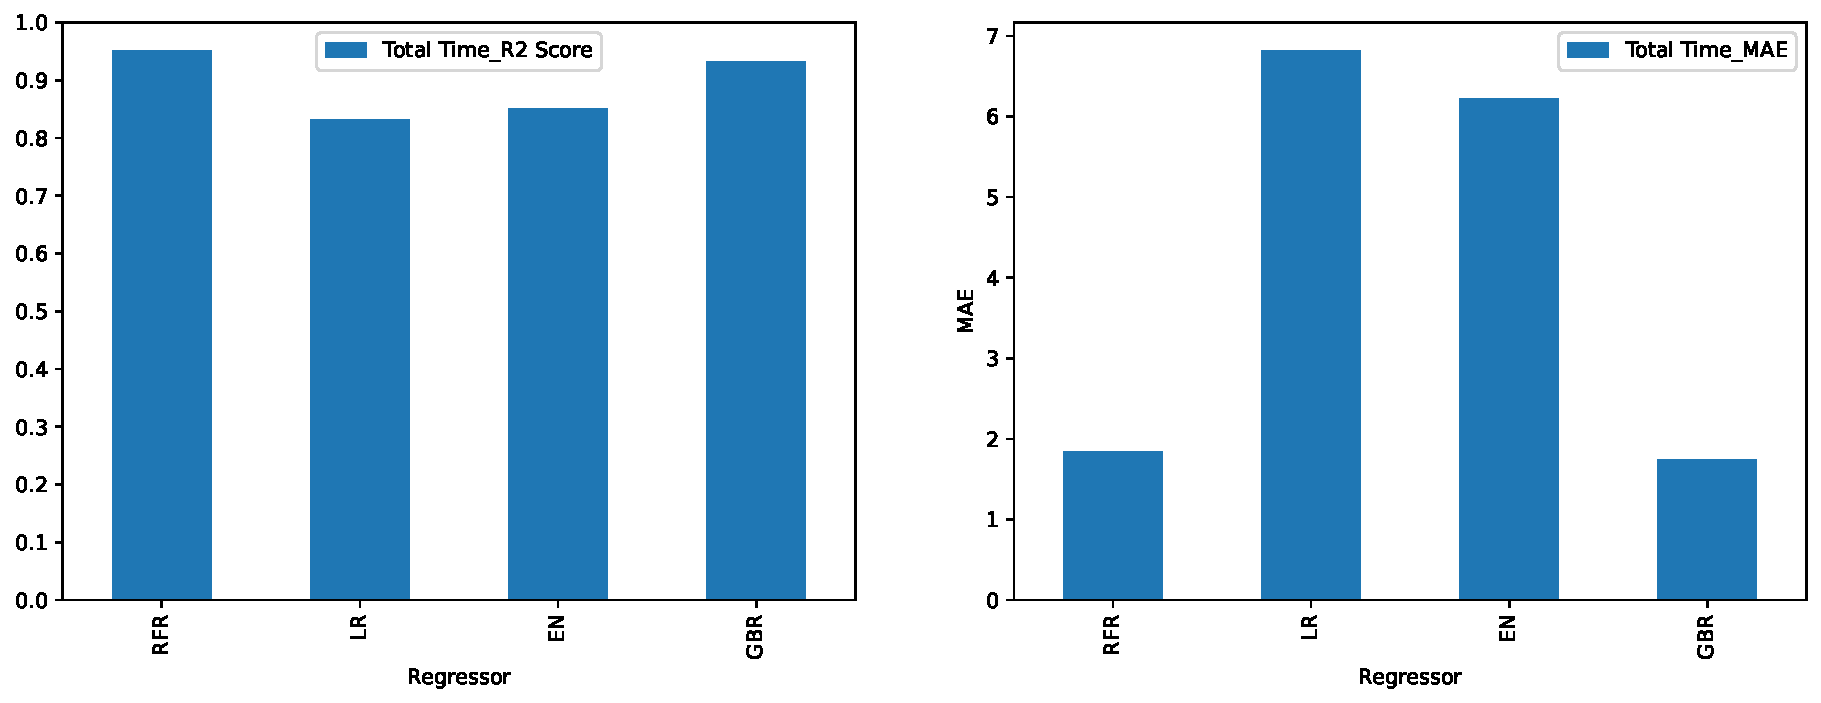
\includegraphics[width=0.48\textwidth]{plots/model_performance_results/random_forest_total_time_results.pdf}
  \caption{Total Time Performance}
\end{figure}

\begin{figure}[ht]
  \centering
  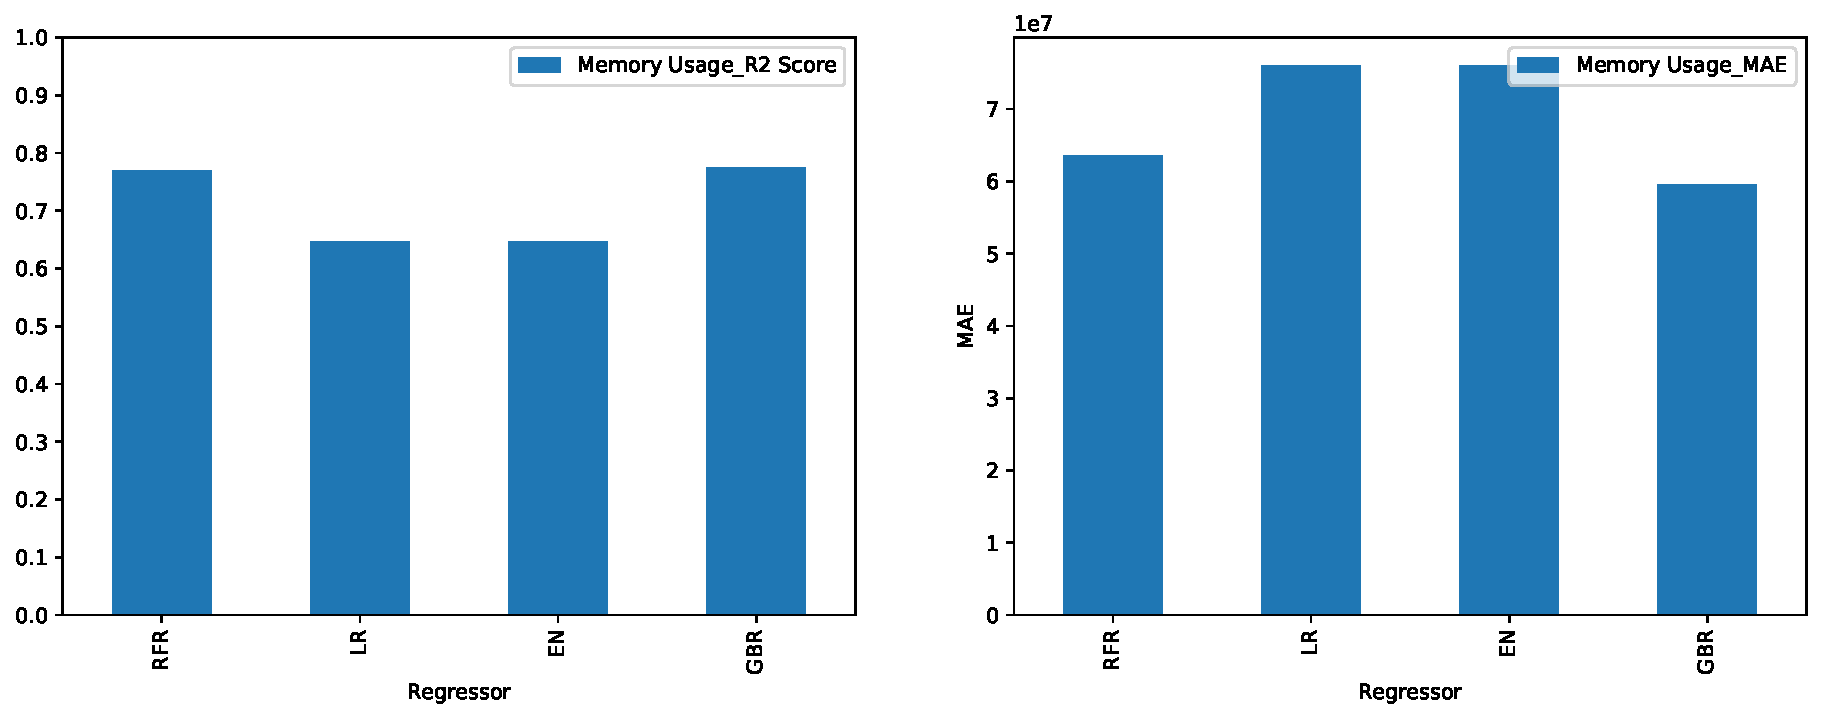
\includegraphics[width=0.48\textwidth]{plots/model_performance_results/random_forest_memory_results.pdf}
  \caption{Memory Usage Performance}
\end{figure}

Similarly, in the graph for memory usage, the Random Forest Regressor and the Gradient Boosting Regressor stood out as the top-performing models, with the former outperforming the latter. Once again, the other models were far behind in terms of performance.

After running a significant number of tests, we found that the Random Forest Regressor had much more stable results across multiple runs. Based on its superior performance, we decided to use the Random Forest Regressor as our final model.

\subsubsection{Kmeans Regression}
The results obtained from the evaluation of total time performance suggest that the Gradient Boosting Regressor exhibits better performance for both R2 and MAE metrics compared to the Random Forest Regressor. Among the evaluated models, the aforementioned models demonstrate the highest accuracy in terms of performance. Conversely, the remaining models exhibit lower levels of accuracy with respect to performance. 
In terms of memory usage, the evaluated models showed similar performance, with no significant differences observed between them. Based on the evaluation results of performance metrics for both total time and memory usage performance the Gradient Boosting Regressor exhibits the best overall performance among the evaluated models.

\begin{figure}[!h]
  \centering
  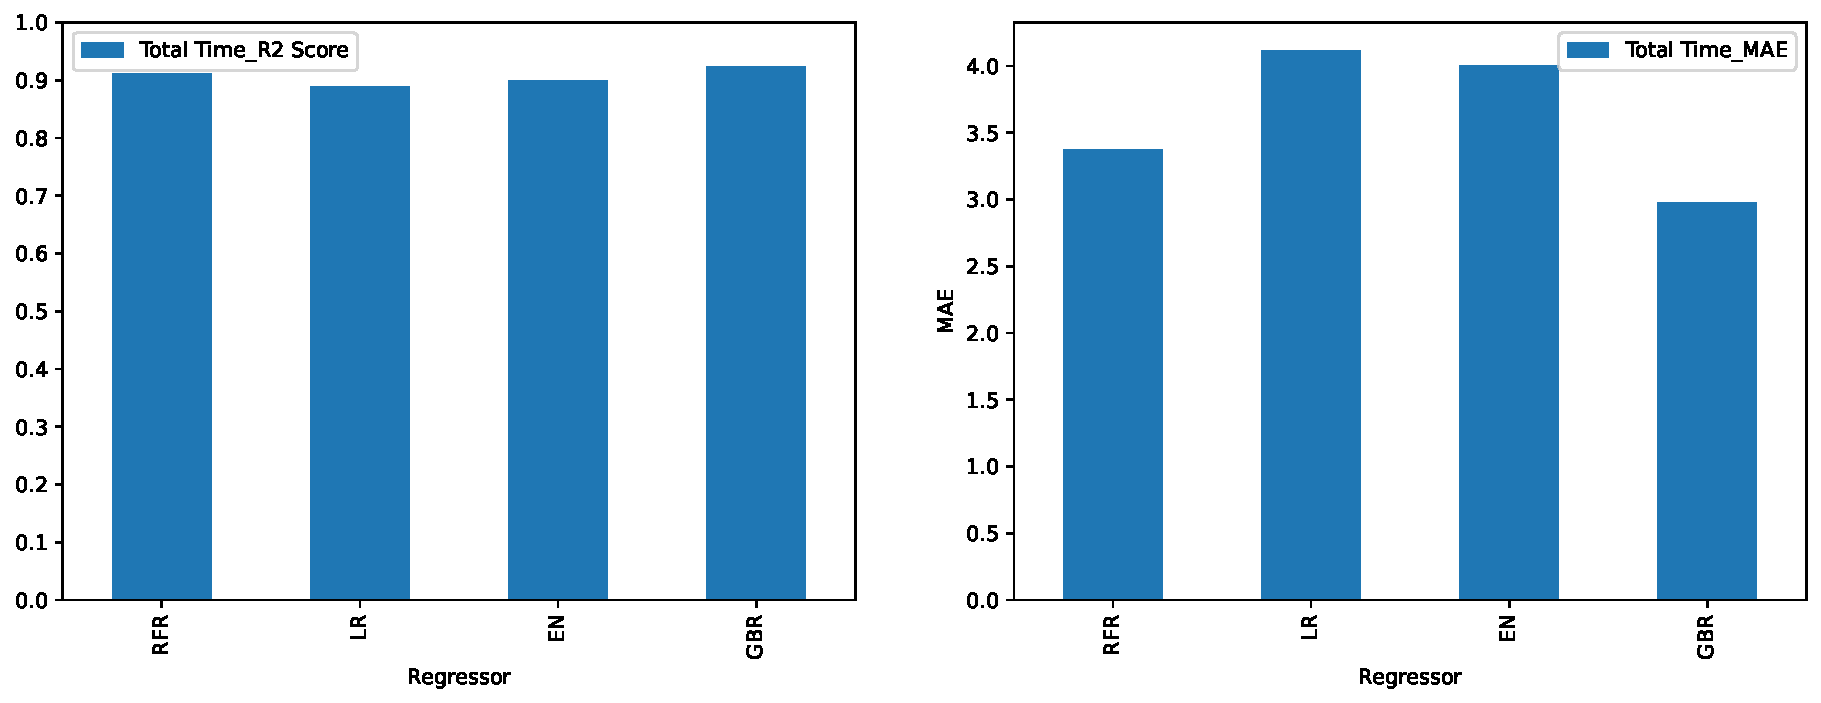
\includegraphics[width=0.48\textwidth]{plots/model_performance_results/kmeans_total_time_results.pdf}
  \caption{Total Time Performance}
\end{figure}

\begin{figure}[ht]
  \centering
  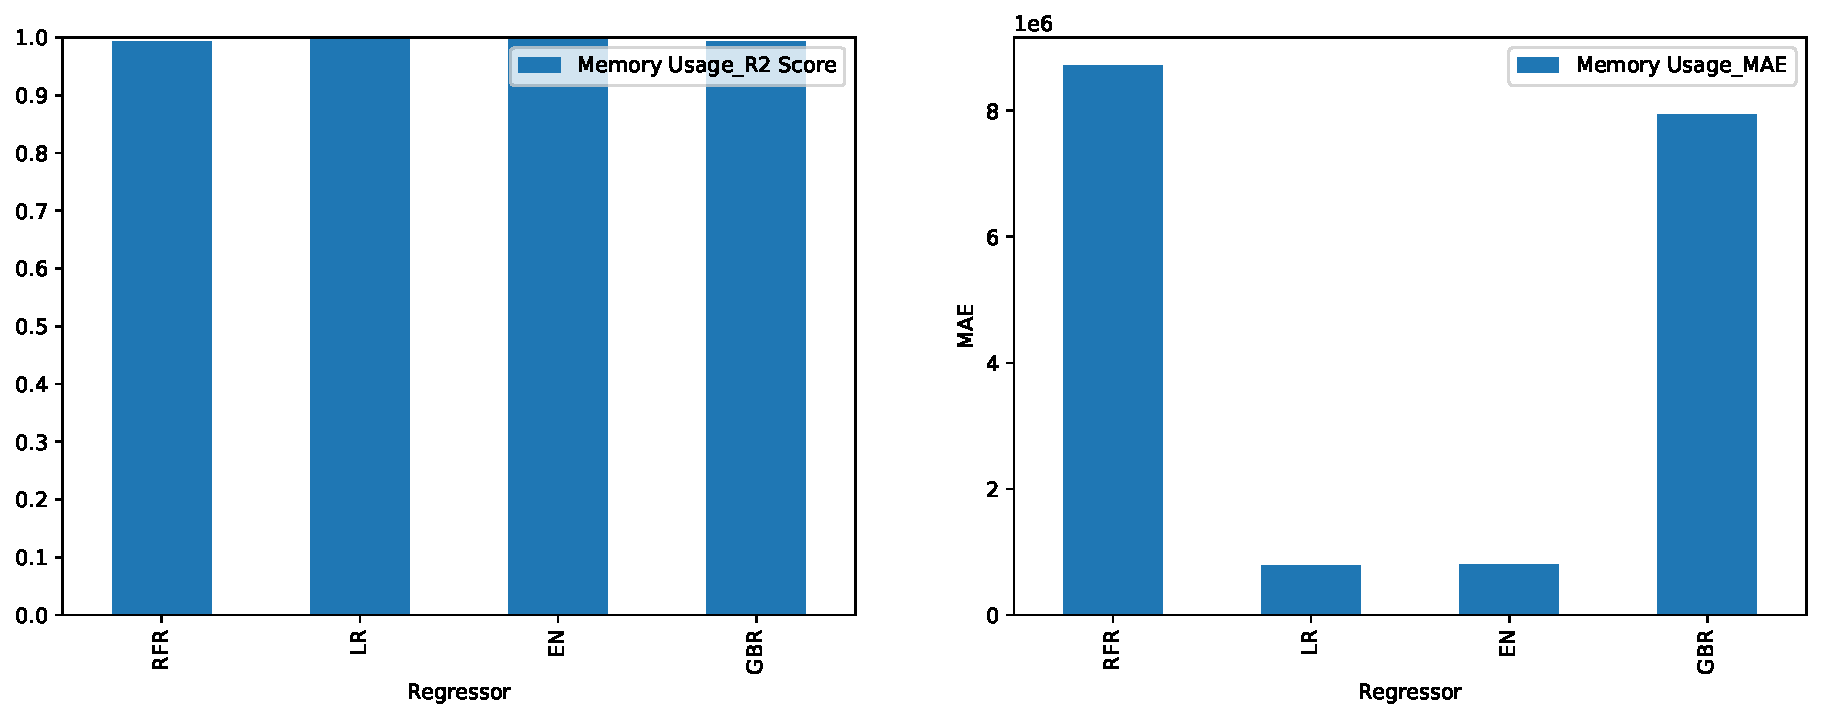
\includegraphics[width=0.48\textwidth]{plots/model_performance_results/kmeans_memory_results.pdf}
  \caption{Memory Usage Performance}
\end{figure}

\subsubsection{Word2Vec Regression}
The evaluation of total time performance revealed that the Linear Regression model outperformed the other models in terms of both R2 and MAE metrics. In terms of memory usage, as we said earlier the data points are not sufficient to train an accurate model, so as we can see from the graphs below the performance for both R2 and MAE is very low. 

\begin{figure}[!h]
  \centering
  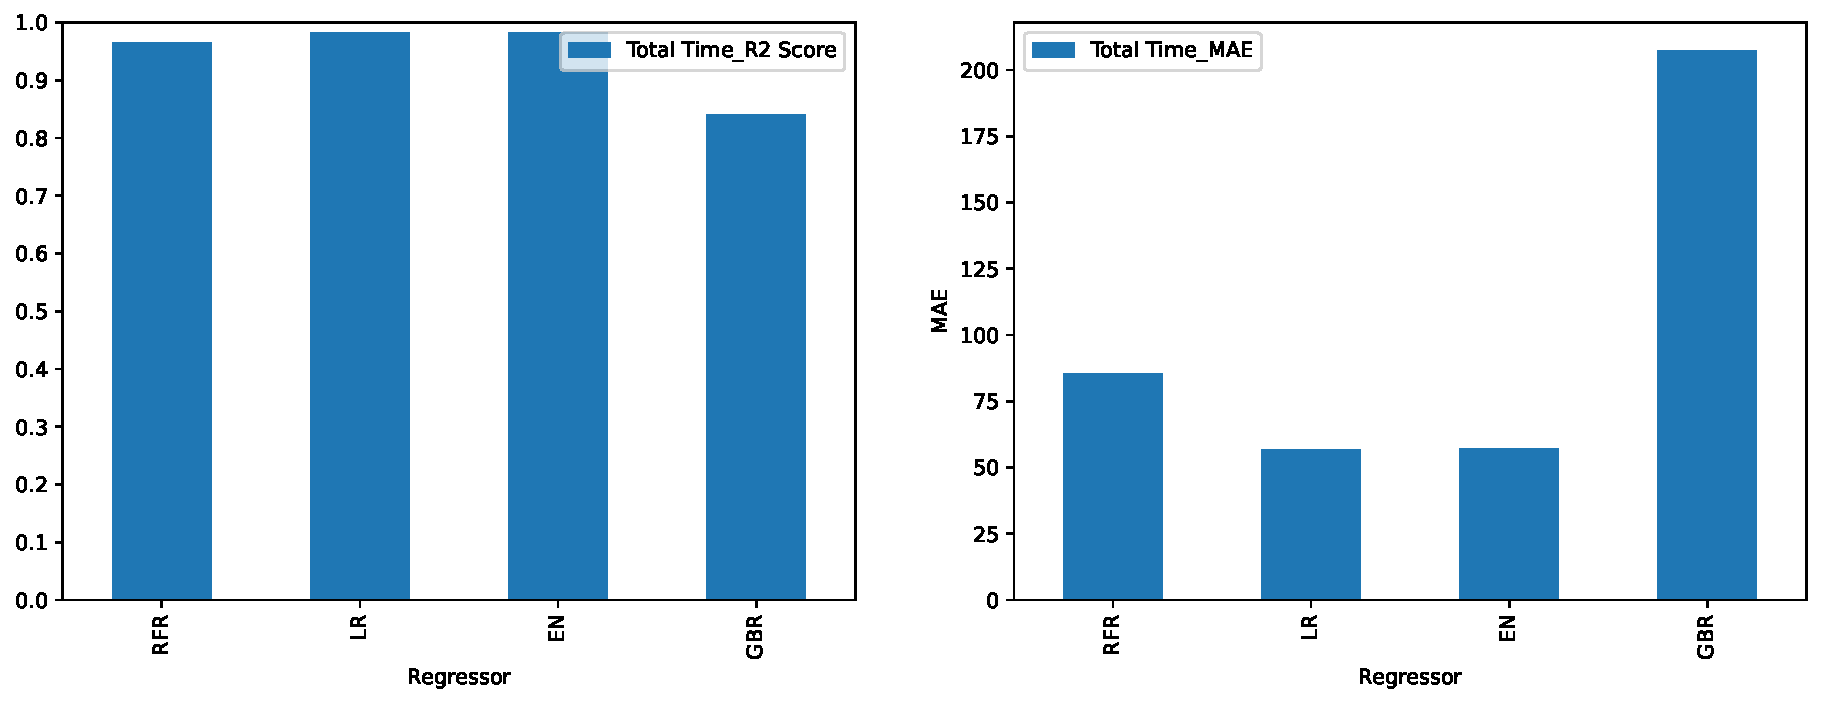
\includegraphics[width=0.48\textwidth]{plots/model_performance_results/Word2Vec_total_time_results.pdf}
  \caption{Total Time Performance}
\end{figure}

\begin{figure}[!h]
  \centering
  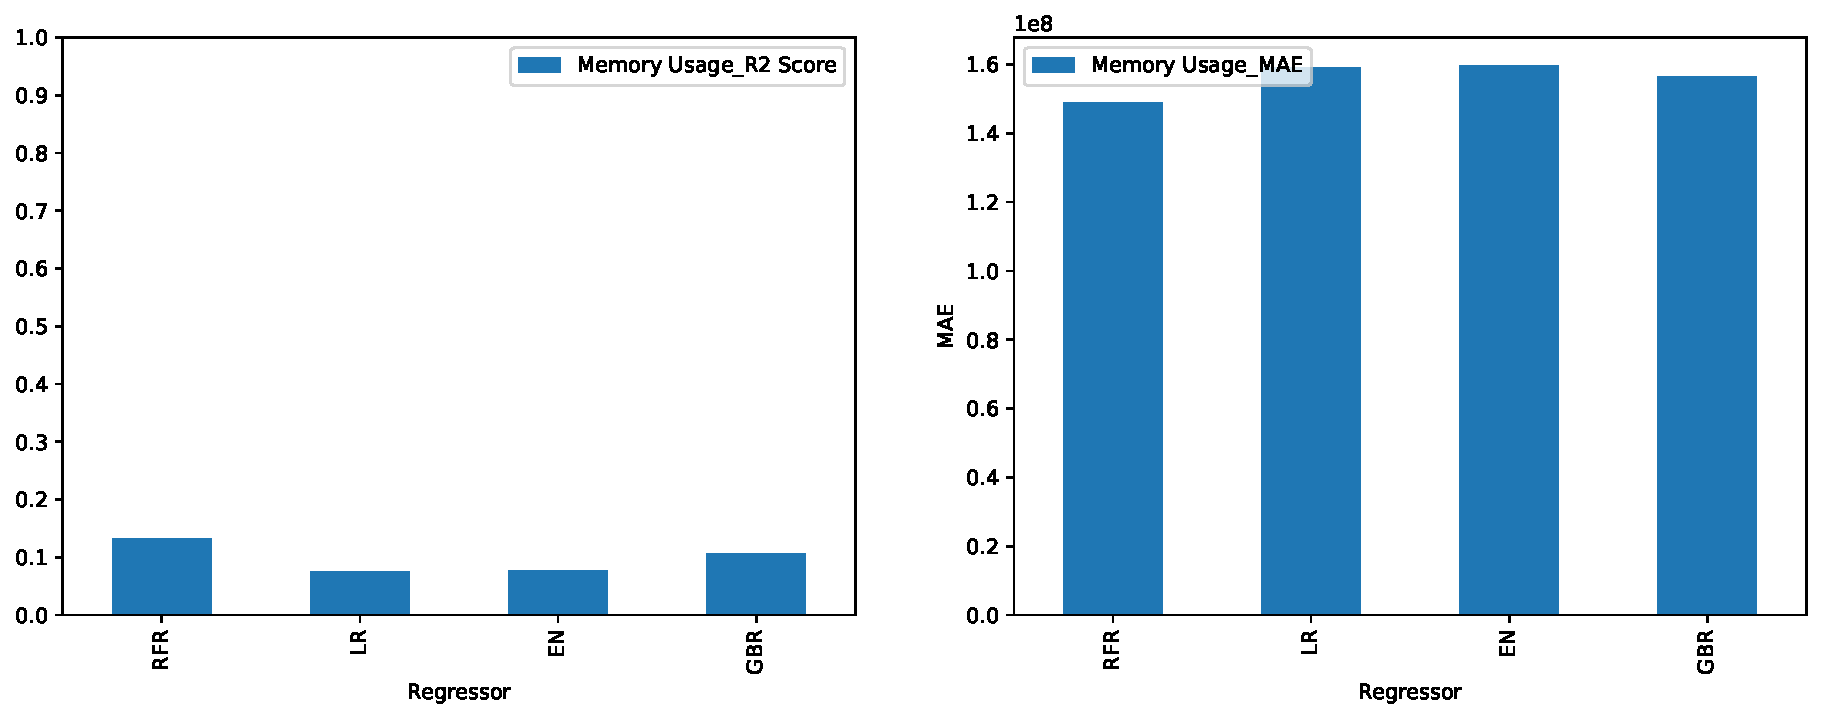
\includegraphics[width=0.48\textwidth]{plots/model_performance_results/Word2Vec_memory_results.pdf}
  \caption{Memory Usage Performance}
\end{figure}



\section{Results and Discussion}

In this study, we explored the inner workings of Apache Spark's MLlib library, which provides a range of algorithms and tools for processing large datasets and building machine learning models. We focused our efforts on three operators, which were k-means clustering, Random Forest Regression, and Word2Vec. We trained models that can accurately predict the behavior of each operator. 

The results of the best models for each operator are presented in Table \ref{tab:ml-operators}.

\begin{table}[ht]
\centering
\caption{Best model and corresponding metrics for each operator}
\label{tab:ml-operators}
\begin{threeparttable}

\begin{tabular}{|c|c|c|c|}
\hline
Operator & Best Model & Total time R2 & Memory usage R2 \\ \hline
K-Means & GBR\tnote{1} & 0.923 & 0.99 \\ \hline
Random Forest & RFR\tnote{2} & 0.952 & 0.77 \\ \hline
Word2vec & LR\tnote{3} & 0.982 & 0.07 \\ \hline
\end{tabular}
\begin{tablenotes}
    \item[1] Gradient Boosting Regressor
    \item[2] Random Forest Regressor
    \item[3] Linear Regressor
  \end{tablenotes}

\end{threeparttable}
\end{table}


Through this study, we have gained a comprehensive understanding of the inner workings of Apache Spark's MLlib library and its ability to process large datasets efficiently while building accurate machine learning models.

ML processing in Spark involves a series of steps, starting with data preparation, where the data is loaded into a DataFrame or RDD and transformed as necessary. Feature extraction is then performed to convert the data into a format suitable for machine learning algorithms. Spark provides several built-in tools for feature extraction.

Once the data is prepared, it can be used to train a machine-learning model. Spark's MLlib library provides a range of algorithms for supervised learning, unsupervised learning, and reinforcement learning. These algorithms are designed to work with distributed data, enabling Spark to process large datasets efficiently. For example, Spark's logistic regression algorithm uses stochastic gradient descent (SGD) to train the model in parallel across multiple nodes in a cluster.


Finally, the trained model can be evaluated using test data to measure its accuracy and performance. Spark provides a range of evaluation metrics for different types of machine learning tasks, including regression metrics such as mean absolute error (MAE) and classification metrics such as accuracy, precision, recall, and F1 score.

In addition to these core steps, Spark's MLlib library provides a range of additional tools and features to support machine learning processing. For example, it includes utilities for working with sparse data, text data, and graph data, as well as tools for model persistence and serialization.

Overall, our study demonstrates the power and flexibility of Apache Spark's MLlib library for machine learning processing. By providing a range of algorithms and tools designed for distributed data, Spark enables efficient processing of large datasets and rapid development of accurate machine learning models. Future work could involve exploring new algorithms and use cases further to demonstrate the capabilities of Spark's ML operators.





\begin{thebibliography}{00}
\bibitem{spark} “Apache SparkTM - Unified Engine for large-scale data analytics.” https://spark.apache.org/
\bibitem{pyspark}  “PySpark Documentation — PySpark 3.3.1 documentation.”https://spark.apache.org/docs/latest/api/python/
\bibitem{scikit-learn}“scikit-learn: machine learning in Python — scikit-learn 1.2.1 documentation.” https://scikit-learn.org/stable/index.html
\bibitem{acropolitan} T. Acropolitan, “Sentence Length Has Declined 75\% in the Past 500 Years,” Medium, Apr. 18, 2018. https://medium.com/@theacropolitan/sentence-length-has-declined-75-in-the-past-500-years-2e40f80f589f
\end{thebibliography}
\vspace{12pt}

\end{document}
